\usetikzlibrary{positioning}

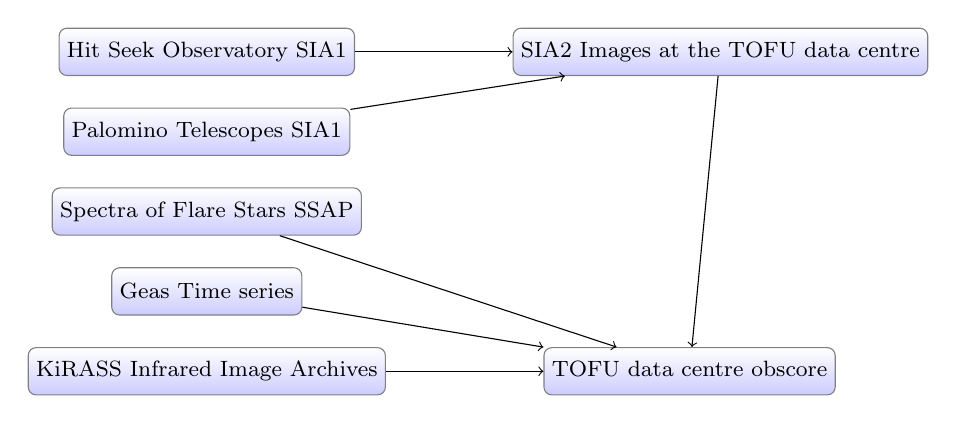
\begin{tikzpicture}[
service/.style={bottom color=blue!20,
  top color=white,
  rounded corners=1mm,
  minimum height=6mm,
  thin,draw=black!50,align=center,
  node distance=4mm and 2cm,
  node font=\footnotesize
}]
\node (s1) [service] {Hit Seek Observatory SIA1};

\node (s2) [service, below=of s1] {Palomino Telescopes SIA1} ;

\node (s3) [service, below=of s2] {Spectra of Flare Stars SSAP} ;

\node (s4) [service, below=of s3] {Geas Time series};

\node (s5) [service, below=of s4] {KiRASS Infrared Image Archives};

\node (s6) [service, right=of s1] {SIA2 Images at the TOFU data centre};

\node (s7) [service, right=of s5] {\strut TOFU data centre obscore};


\draw [black,->] (s1) to (s6);
\draw [black,->] (s2) to (s6);
\draw [black,->] (s3) to (s7);
\draw [black,->] (s4) to (s7);
\draw [black,->] (s5) to (s7);
\draw [black,->] (s6) to (s7);
\end{tikzpicture}
